\newcommand{\nonblockedMethodFigure}{
\begin{figure}[h]
    \centering
    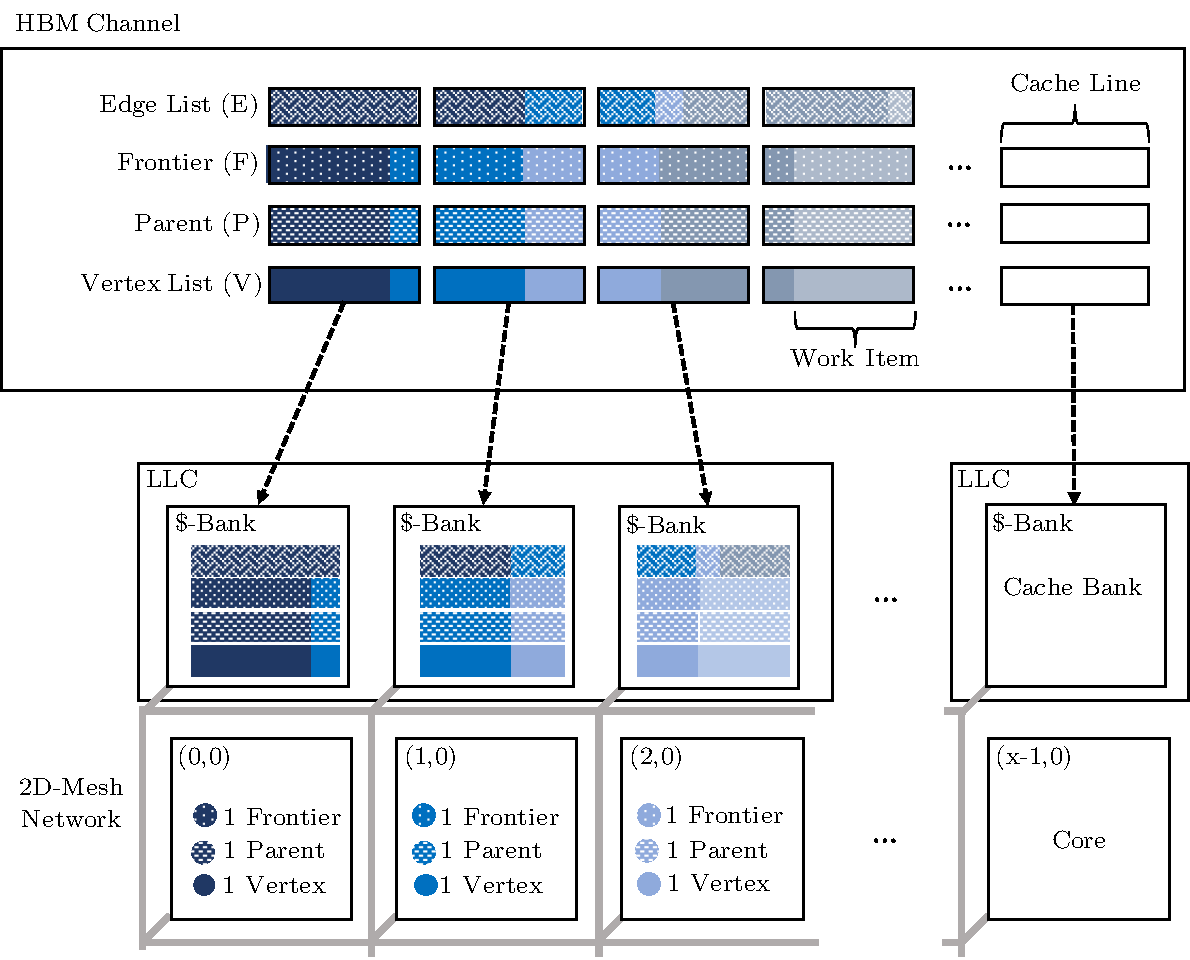
\includegraphics[scale=0.7]{graphit-figures/non-blocked.pdf}
    \caption{Data layout of BFS on the manycore. Data resides in HBM main memory and is cached in LLC. Each core is assigned work items sized without alignment consideration. Cores request single words of data on demand when needed. }
    \label{pap:generals:sec:method:sub:blocked:fig:non-blocked}
\end{figure}
}

\newcommand{\blockedMethodFigure}{
\begin{figure}[t]
    \centering
    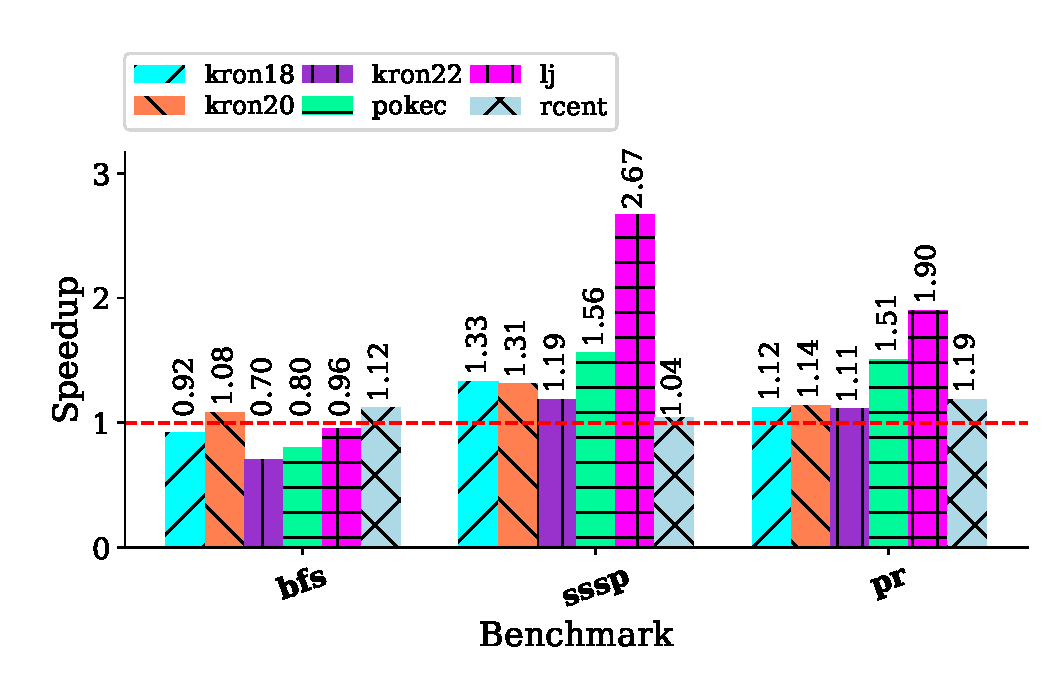
\includegraphics[scale=0.7]{graphit-figures/blocked.pdf}
    \caption{Data layout of BFS with blocked accesses. Cores are assigned cache aligned work items. Cores prefetch entire line-sized blocks of data to hide request latency.}
    \label{pap:generals:sec:method:sub:blocked:fig:blocked}
\end{figure}
}

\newcommand{\combinedBlockingFigure}{
\begin{figure*}[t!]
    \centering
    \subfloat[Non-Blocked Accesses]{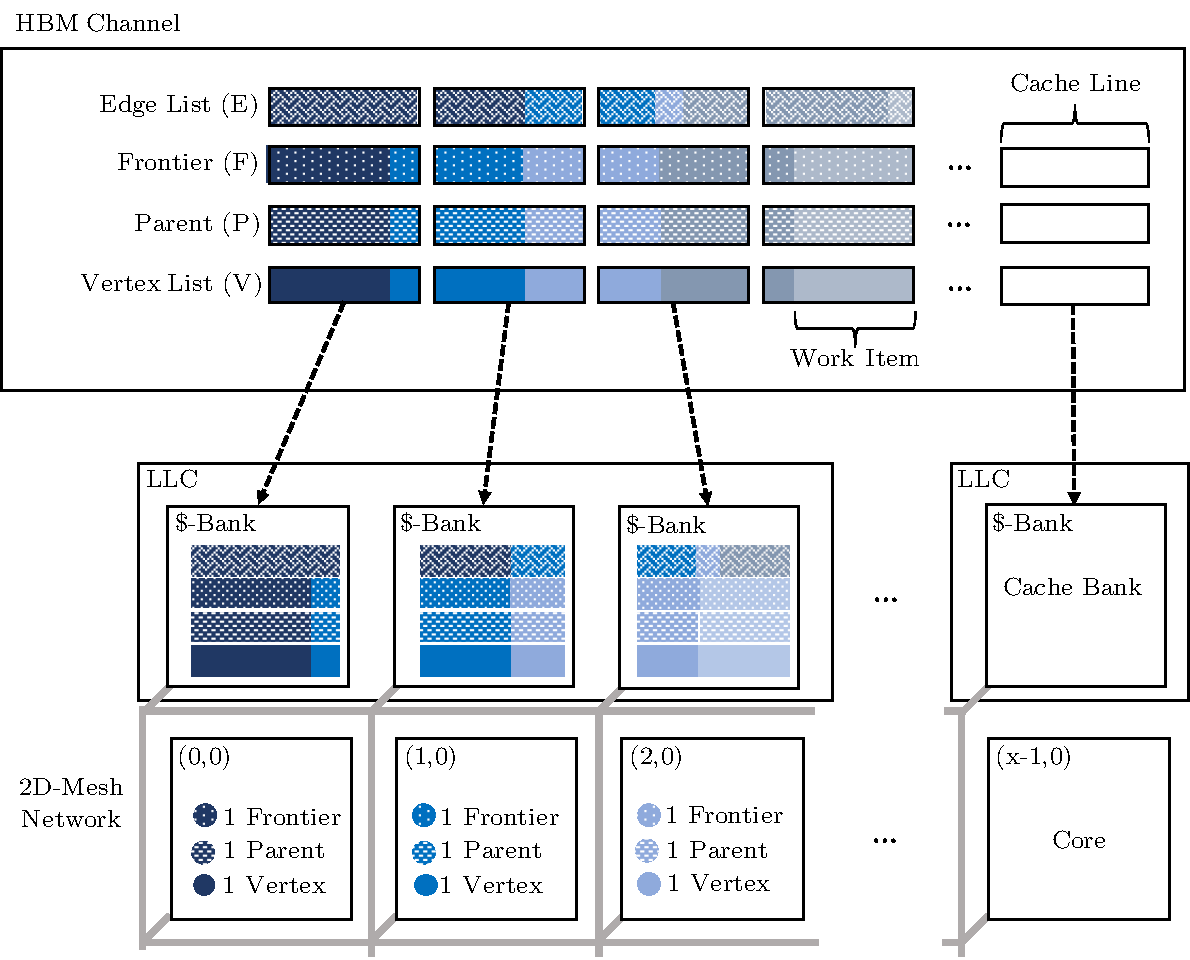
\includegraphics[scale=0.7]{graphit-figures/non-blocked.pdf}}
    \qquad
    \subfloat[Blocked Accesses]{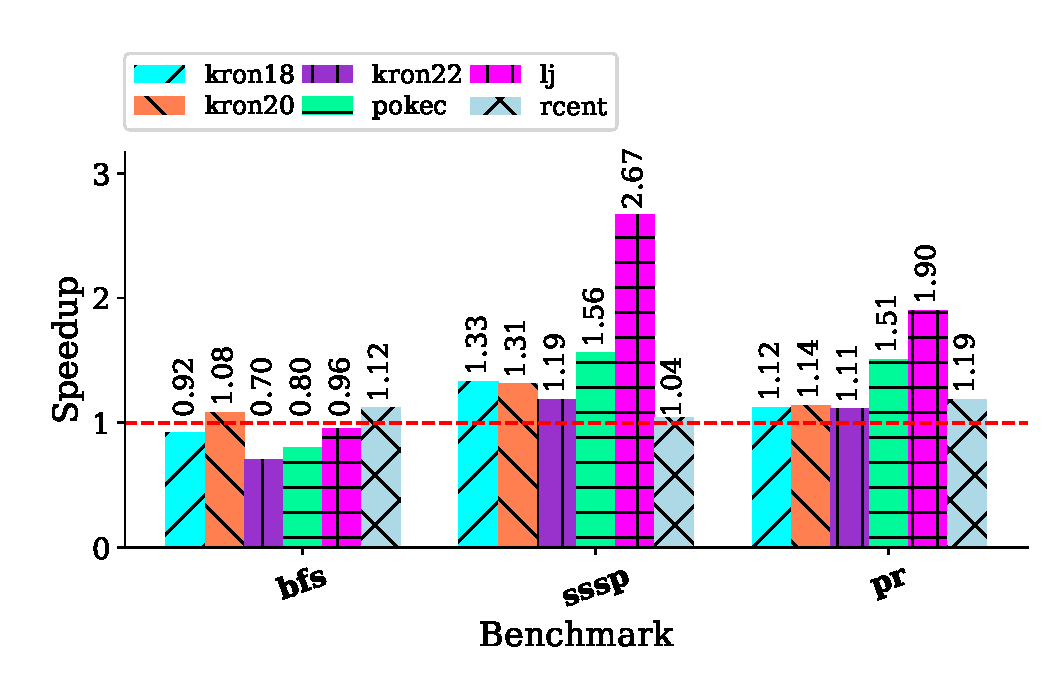
\includegraphics[scale=0.7]{graphit-figures/blocked.pdf}}
    \caption{Data layout of BFS on the manycore. Data resides in HBM main memory and is cached in LLC. In the baseline implementation, each cores are assigned work items sized without alignment consideration and request single words of data on demand when needed. With the blocked access optimization, cores are assigned cache aligned work items and prefetch entire line-sized blocks of data to hide request latency.}
    \label{pap:generals:sec:method:sub:blocked:fig:blocking}
\end{figure*}
}

\newcommand{\edgeAwareMethodFigure}{
\begin{figure}
    \centering
    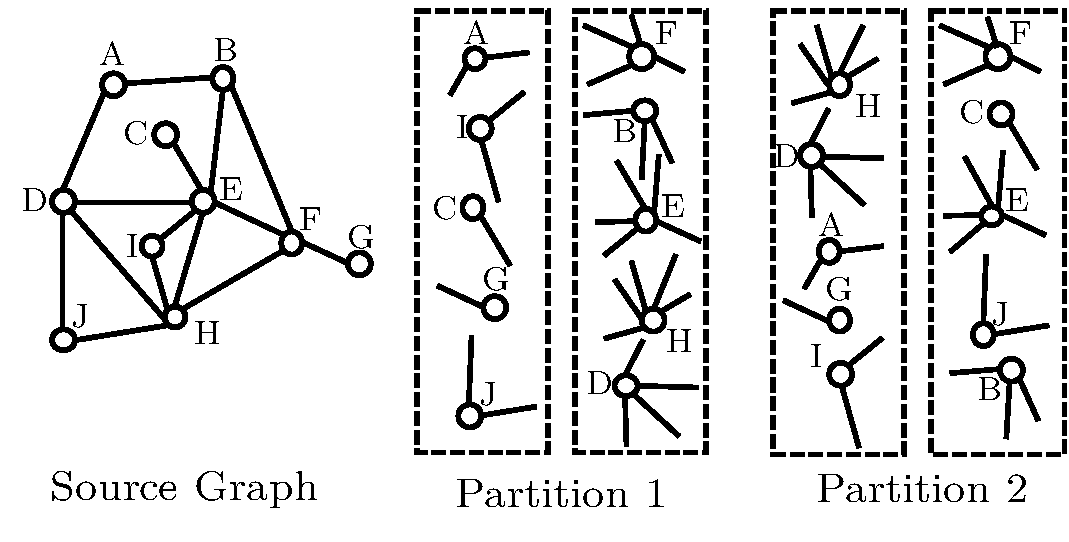
\includegraphics[scale=0.6]{graphit-figures/edge-aware.pdf}
    \caption{Depiction of vertex-based and edge-aware vertex-based partitioning. Partition 1 shows an example vertex-based partitioning between two cores, and Partition 2 shows an example edge-aware partitioning that provides a better workload balance between the two cores.}
    \label{fig:edgeaware}
\end{figure}
}
\newcommand{\edgeAwareMethodAlgorithm}{
\begin{figure}
\centering
\begin{algorithmic}[1]
\Function{Recursive Range}{$start, end$}
\If {$index[end] - index[start] < grain size$}
    \State $core.start \gets start$
    \State $core.end \gets end$
\Else 
    \State $recursive range (start, end/2)$
    \State $recursive range (end/2, start)$
\EndIf
\EndFunction
\end{algorithmic}
\caption{Pseudocode for the recursive call portion of the edge-aware vertex partitioning scheme.}
    \label{alg:edge-aware}
\end{figure}
}
\newcommand{\pushVPullMethodFigure}{
\begin{figure}
    \centering
    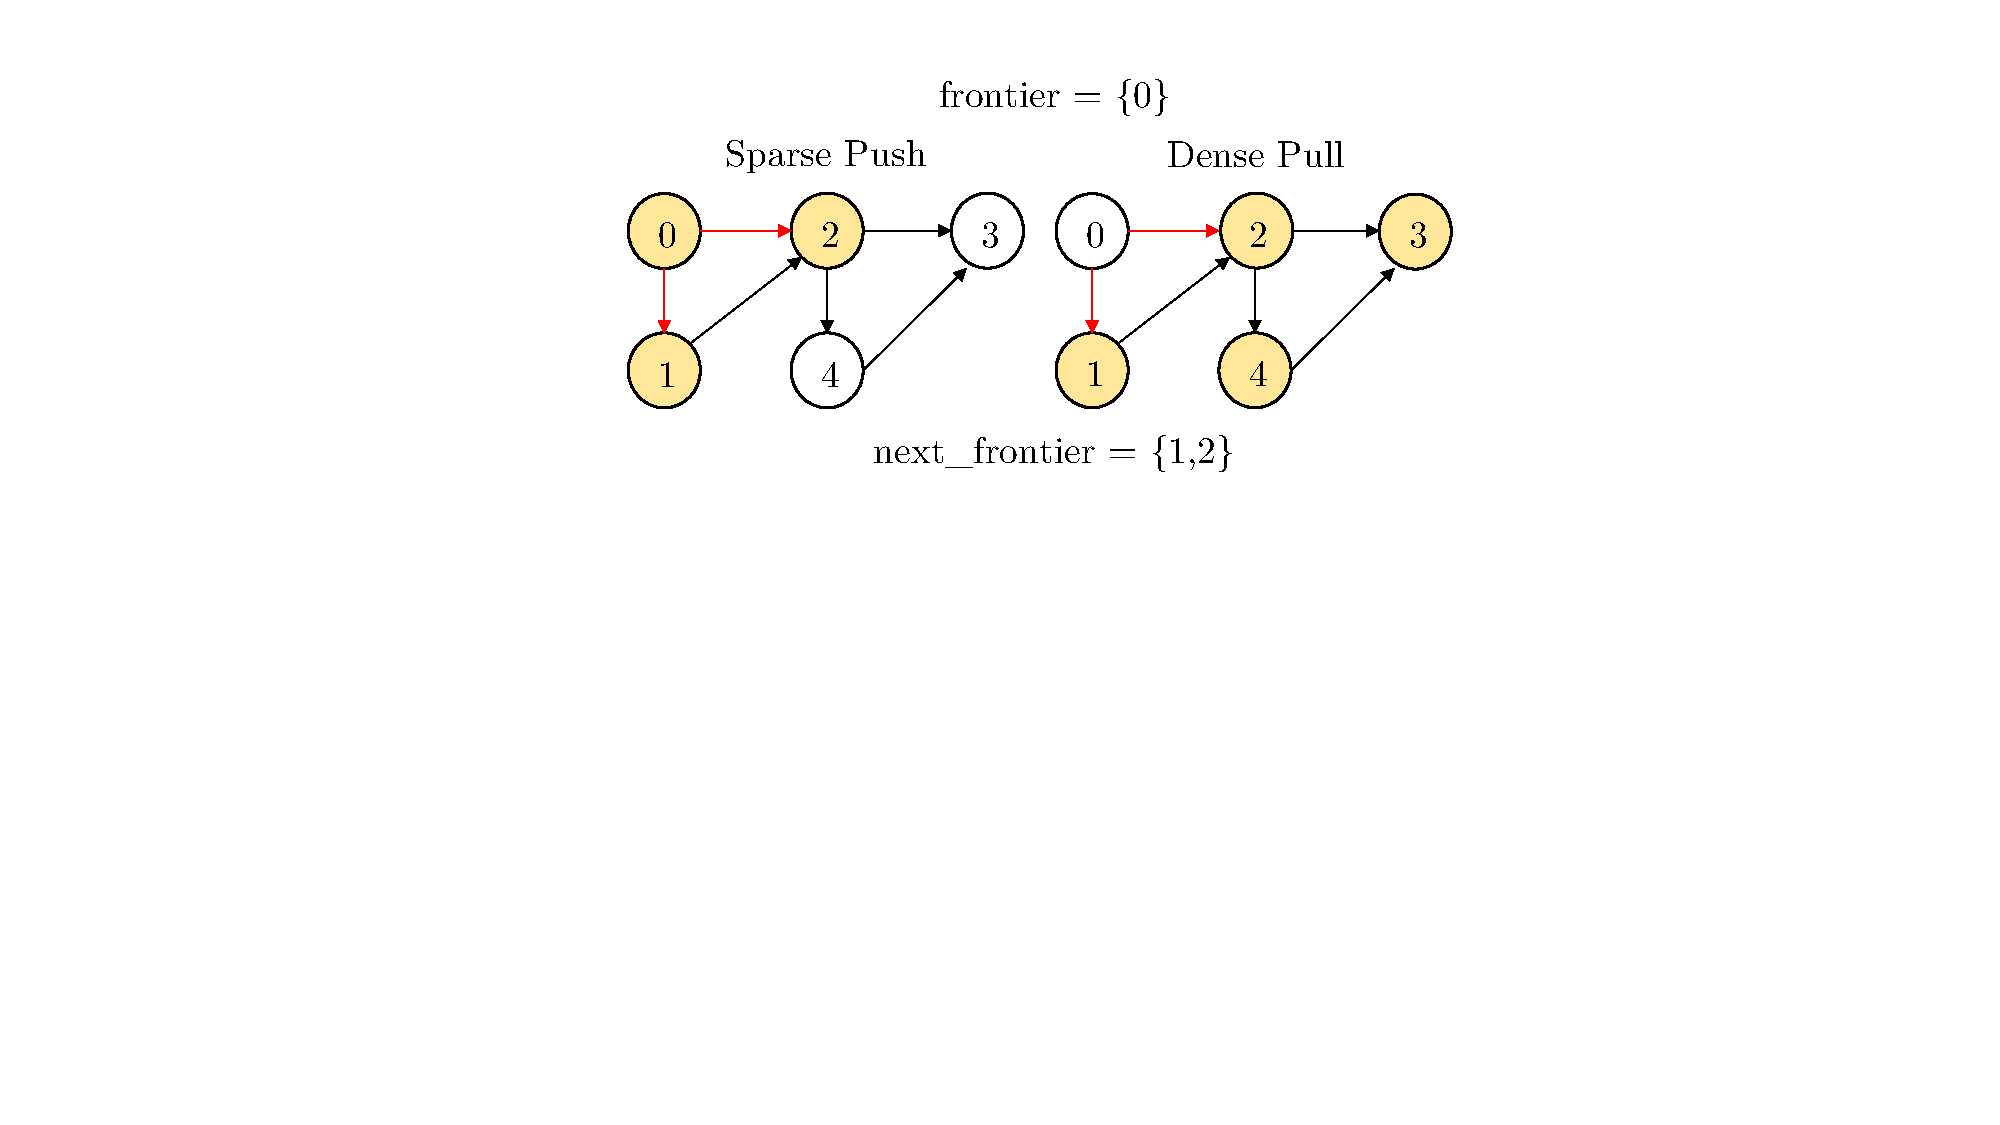
\includegraphics[scale=0.7]{graphit-figures/push_v_pull_fig.pdf}
    \caption{Representation of one iteration of BFS in both the \textsc{Push} and \textsc{Pull} directions. Nodes highlighted in yellow are visited during the iteration. Edges in red are edges that are traversed during execution.}
    \label{fig:pushpull}
\end{figure}
}